\chapter{Offuscamento}

In questa capitolo si ha l'obiettivo di ingannare i tool di figerprinting, portandoli ad un risultato errato. Più precisamente, si ha lo scopo di modificare parametri di Kali per ottenere il riconoscimento di Windows.
\\
Non essendo Windows 11 presente nel database di Nmap e non potendo quindi essere un risultato del fingerprinting, si cercherà di portare i tool all'individuazione della sua versione precedente, ovvero Windows 10.

\section{Algoritmo utilizzato da Nmap} \label{algoritmi}
Prima di procedere occorre precisare il funzionamento dell'algoritmo di Nmap per il riconoscimento dei sistemi operativi. Questo avviene secondo un meccanismo di punteggi che viene dato ad ogni test effettuato, specificato nella prima entry del database. I test che non ottengono alcun risultato utile non vengono conteggiati nel totale dei punti.
A questo punto, vi sono due possibili situazioni:
\begin{itemize}
	\item Se i risultati dei test combaciano perfettamente con quelli di una entry del database, allora quella verrà mostrata come risultato finale,
	\item Se i risultati dei test non coincidono con nessun sistema operativo, allora verranno calcolati i punti di ogni test soddisfatti per ogni sistema; quello con cui è stato realizzato un numero maggiore di punti sarà quello mostrato.
\end{itemize}

Segue l'elenco di test con il relativo punteggio \cite{punti_nmap}:

\begin{lstlisting}[caption={Punteggi che Nmap attrribuisce ad ogni test}]
	MatchPoints
	SEQ(SP=25%GCD=75%ISR=25%TI=100%CI=50%II=100%SS=80%TS=100)
	OPS(O1=20%O2=20%O3=20%O4=20%O5=20%O6=20)
	WIN(W1=15%W2=15%W3=15%W4=15%W5=15%W6=15)
	ECN(R=100%DF=20%T=15%TG=15%W=15%O=15%CC=100%Q=20)
	T1(R=100%DF=20%T=15%TG=15%S=20%A=20%F=30%RD=20%Q=20)
	T2(R=80%DF=20%T=15%TG=15%W=25%S=20%A=20%F=30%O=10%RD=20%Q=20)
	T3(R=80%DF=20%T=15%TG=15%W=25%S=20%A=20%F=30%O=10%RD=20%Q=20)
	T4(R=100%DF=20%T=15%TG=15%W=25%S=20%A=20%F=30%O=10%RD=20%Q=20)
	T5(R=100%DF=20%T=15%TG=15%W=25%S=20%A=20%F=30%O=10%RD=20%Q=20)
	T6(R=100%DF=20%T=15%TG=15%W=25%S=20%A=20%F=30%O=10%RD=20%Q=20)
	T7(R=80%DF=20%T=15%TG=15%W=25%S=20%A=20%F=30%O=10%RD=20%Q=20)
	U1(R=50%DF=20%T=15%TG=15%IPL=100%UN=100%RIPL=100%RID=100%RIPCK=100%
	RUCK=100%RUD=100)
	IE(R=50%DFI=40%T=15%TG=15%CD=100)
\end{lstlisting}

Come si può notare, alcuni test hanno un valore maggiore rispetto ad altri per la frequenza con cui vengono svolti. Ad esempio il test T, che controlla il valore del TTL iniziale, viene effettuato nove volte mentre il test CD che verifica il campo code nel protocollo ICMP viene effettuato una sola volta.
Questa è una delle ragioni che spiega la discrepanza tra i punteggi attribuiti ai diversi test che vengono svolti.
Un ulteriore esempio di quanto appena affermato si può trovare tra i test della riga OPS (effettuati sulle opzioni TCP) e i test sulla riga U1, riguardanti il protocollo UDP.


\section{Modifiche al file sysctl.conf}
Per ottenere un sistema operativo differente, occorre modificare alcuni parametri del file sysctl.conf in modo da ottenere i valori di Windows.
La prima modifica riguarda il campo del TTL; variarlo da 64 a 128 consente di ingannare il test T, che calcola il valore iniziale di questo campo. La modifica vale per tutti i pacchetti che verranno inviati, quindi questo consente di spostare un grande quantità di punti a favore del riconoscimento di Windows, essendo il test ripetuto per molti pacchetti.

\begin{lstlisting}[caption={Modifica al campo TTL nel file sysctl.conf}, label=listing_ttl]
	net.ipv4.ip_default_ttl=128
\end{lstlisting}

Un'ulteriore modifica può essere effettuata per quanto riguarda il flag ECN, la cui differenza è stata spiegata nella sezione \ref{tab:ECN}. Questo riguarda i test della quarta riga, in cui quello specifico per la notifica esplicita di congestione ha un valore di 100 punti.

\begin{lstlisting}[caption={Modifica al campo ECN nel file sysctl.conf}]
	net.ipv4.tcp_ecn=0
\end{lstlisting} 

Il valore 0 significa che l'host non può accettare né inizializzare l'utilizzo del flag ECN. Il comportamento in risposta a determinati pacchetti "patologici" è ora simile a quello di Windows.

Si può inoltre procedere modificando il valore della Windows Size massima, causando di conseguenza un cambiamento del valore del Window Scaling Factor, da 7 a 8. 
La riga scritta nel file è la seguente:

\begin{lstlisting}[caption={Modifica alla Windows Size massima nel file sysctl.conf}, label=listingscaling]
	net.core.rmem_max = 8388608
\end{lstlisting}

Questa modifica, presa singolarmente, non influenza il risultato del fingerprinting in quanto questo campo è contenuto all'interno delle TCP options, che vengono valutate in maniera aggregata. Servono quindi ulteriori modifiche che verranno illustrate successivamente.

\section{Modifiche tramite nftables}
La modifica dei pacchetti in uscita dall'host di cui si vuole effettuare il fingerprinting tramite nftables consente il cambiamento del comportamento solo in determinate situazioni; di particolare interesse sono quelle riguardanti i probe di Nmap.
\\
La differenza mostrata alla tabella \ref{tab:code} è oggetto di uno dei test effettuati da Nmap. Quest'ultimo, infatti, invia un pacchetto \textit{echo request} con campo \textit{code} impostato a 9, e valuta la risposta ricevuta.
Questa dovrebbe essere zero nel caso di un \textit{echo reply}, ma questo comportamento è in realtà dipendente dal sistema operativo in utilizzo.
Manipolare i pacchetti echo reply in uscita per modificare il campo code nel caso questo sia 9 consente la variazione del risultato del test effettuato da Nmap. L'alto valore in termini di punteggio assegnato a questo test rende questa modifica molto importante ai fini dell'offuscamento.\\
Il comando per ottenere questo comportamento è contenuto nel file nftables.conf, nella tabella output.

\begin{lstlisting}[caption={Modifica del campo code in caso di test Nmap}, label=codice_icmp]
	icmp type 0 icmp code 9 icmp code set 0
\end{lstlisting}

Esaminando il database di Nmap, ci si accorge che vi è una differenza nel Window Size tra Kali e Windows 10. Modificare questo campo permette quindi di falsificare un altro test eseguito da Nmap, contribuendo quindi alla realizzazione dell'offuscamento.
Si procede dunque ad impostare la Window Size come descritta nel database.

\begin{lstlisting}[caption={Modifica della Window Size}, label=listingsize]
	tcp window != 0x2000 tcp window set 0x2000
\end{lstlisting}

Attuando tutte le modifiche elencate fino a questo punto, l'output di Nmap risulta essere il seguente:

\begin{figure}[H]
	\centering
	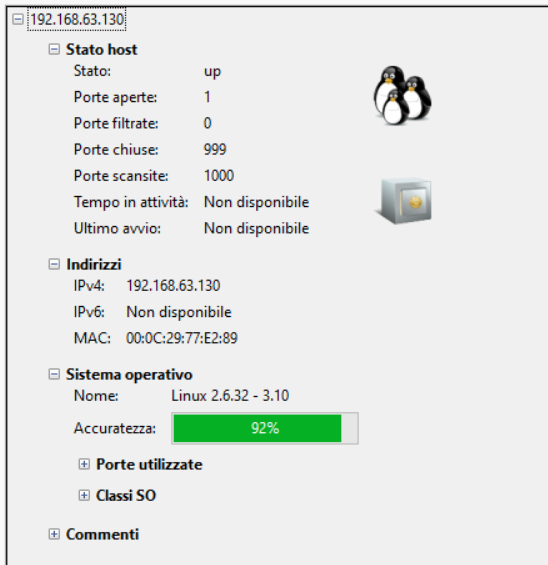
\includegraphics[scale=0.85]{figures/primo_nmap.png}
	\caption{Risultato di Nmap}
	\label{primo_nmap}
\end{figure}

Come si può evincere dall'immagine, viene riconosciuta una versione di Linux non corrispondente a quella attualmente in uso. Quest'operazione è possibile effettuarla eseguendo il seguente comando sul terminale:
\begin{lstlisting}[caption={Comando per mostrare la versione attualmente in uso}]
	hostnamectl
\end{lstlisting}
Visionando ulteriormente il risultato, si può notare come siano state rilevate sia porte aperte che porte chiuse. Questo consente una maggiore precisione nel fingerprinting perché i test vengono effettuati su entrambe le condizioni delle porte, individuate precedentemente tramite port scanning; è quindi logico che evitare questa situazione consente di influenzare parecchio il risultato del fingerprinting.
\\
Per poter evitare la situazione appena descritta, occorre quindi che l'host rifiuti tutti i pacchetti ricevuti che non abbiano come porta destinazione 80 (Well-Known port corrispondente al protocollo applicativo HTTP).
\\
Si procede quindi inserendo una semplice regola nella tabella input delle nftables:

\begin{lstlisting}[caption={Regola per il blocco di tutti i pacchetti ricevuti non diretti alla porta 80}]
	tcp dport != 80 drop
\end{lstlisting}

Con l'utilizzo di questa regola, tutte le porte che prima risultavano \textit{chiuse} ora risultano \textit{filtrate}; la mancanza di test per pacchetti inviati alle porte filtrate influenza pesantemente il risultato del fingerprinting.

\begin{figure}[H]
	\centering
	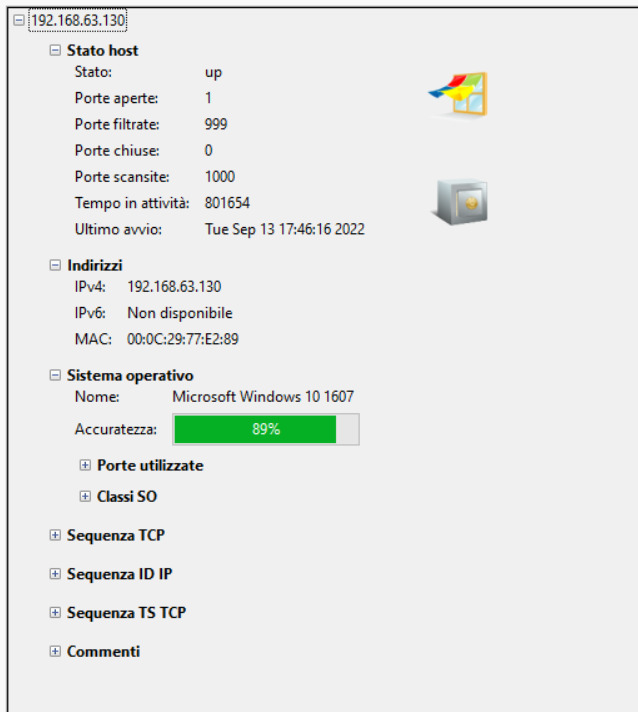
\includegraphics[scale=0.85]{figures/windows_nmap.png}
	\caption{Risultato di Nmap dopo il filtraggio dei pacchetti non diretti alla porta 80}
	\label{windows_nmap}
\end{figure}

Si tratta di un fingerprinting che Nmap definisce "aggressivo", dovuto al fatto che parecchi test non è stato possibile eseguirli; anche per questa ragione la percentuale di sicurezza di Nmap è 89\%, un valore elevato ma che testimonia l'assenza di una certezza assoluta.\\
Si può quindi affermare che la mancanza di porte chiuse in favore di quelle filtrate sia una strategia utile a contrastare il fingerprinting attivo, diminuendo di fatto i controlli che possono essere effettuati sui pacchetti.

\section{Offuscamento da fingerprinting passivo}
Le tecniche seguite per ingannare i tool di fingerprinting passivo non presentano numerose differenze rispetto a quelle della sezione 4.3; vi è però da considerare il fatto che i pacchetti analizzati non sono ricevuti in risposta a determinati probe.
Questo rende alcune regole impostate precedentemente non più funzionanti, come ad esempio la \ref{codice_icmp}; in questo caso, infatti, l'host non riceve alcun pacchetto echo request con campo code impostato a 9.

Segue l'analisi del database di p0f, presente nel file al percorso /etc/p0f/p0f.fp, con i risultati dei test e le possibilità per un eventuale offuscamento. L'elenco dei campi è specificato nella documentazione offerta da p0f \cite{database_p0f}.
\begin{lstlisting}[caption={Fingerptinting TCP con p0f}]
[tcp:request]

sig = ver:ittl:olen:mss:wsize,scale:olayout:quirks:pclass

label = s:unix:Linux:3.11 and newer
sig   = *:64:0:*:mss*20,10:mss,sok,ts,nop,ws:df,id+:0
sig   = *:64:0:*:mss*20,7:mss,sok,ts,nop,ws:df,id+:0

label = s:win:Windows:XP
sig   = *:128:0:*:16384,0:mss,nop,nop,sok:df,id+:0
sig   = *:128:0:*:65535,0:mss,nop,nop,sok:df,id+:0
sig   = *:128:0:*:65535,0:mss,nop,ws,nop,nop,sok:df,id+:0
sig   = *:128:0:*:65535,1:mss,nop,ws,nop,nop,sok:df,id+:0
sig   = *:128:0:*:65535,2:mss,nop,ws,nop,nop,sok:df,id+:0
\end{lstlisting}

Il primo valore di cui si può notare la differenza si trova in corrispondenza del campo \textit{ittl}, corrispondente al Time To Live iniziale.
Si tratta di un campo che è possibile modificare per ottenere un offuscamento modificando il file sysctl.conf come descritto al listing \ref{listing_ttl}.
Per quanto riguarda il campo wsize (riferito al Window Size), anche qui vi sono delle diversità, così come per il valore del Window Scaling; entrambi questi valori sono modificabili tramite le regole descritte al listing \ref{listingsize} e \ref{listingscaling}.
Infine, si può riscontrare una differenza nelle opzioni TCP (campo olayout); queste, infatti, non vengono valutate solamente sul loro utilizzo ma anche nell'ordine in cui queste vengono presentate. È evidente che l'ordinamento utilizzato dai due sistemi operativi sia differente, ma purtroppo non è stato trovato alcun modo per modificare quest'ultime.\\
Nonostante ciò, p0f non possiede un meccanismo di punteggio come Nmap, e non mostra il sistema operativo più simile a quello effettivamente testato. Questa caratteristica consente quindi di ottenere un offuscamento anche apportando modifiche minime al fine di determinare un nuovo comportamento del sistema operativo che non sia riconducibile a nessuna riga del database.

P0f analizza inoltre anche il fingerprinting del secondo pacchetto di un handshake TCP (SYN+ACK) \cite{database_p0f}.

\begin{lstlisting}[caption={Database fingerprinting per pacchetti SYN+ACK dell'handshake TCP}]	
	sig = ver:ittl:olen:mss:wsize,scale:olayout:quirks:pclass

	label = s:unix:Linux:3.x
	sig   = *:64:0:*:mss*10,0:mss:df:0
	sig   = *:64:0:*:mss*10,0:mss,sok,ts:df:0
	sig   = *:64:0:*:mss*10,0:mss,nop,nop,ts:df:0
	sig   = *:64:0:*:mss*10,0:mss,nop,nop,sok:df:0
	sig   = *:64:0:*:mss*10,*:mss,nop,ws:df:0
	sig   = *:64:0:*:mss*10,*:mss,sok,ts,nop,ws:df:0
	sig   = *:64:0:*:mss*10,*:mss,nop,nop,ts,nop,ws:df:0
	sig   = *:64:0:*:mss*10,*:mss,nop,nop,sok,nop,ws:df:0
	
	label = s:win:Windows:7 or 8
	sig   = *:128:0:*:8192,0:mss:df,id+:0
	sig   = *:128:0:*:8192,0:mss,sok,ts:df,id+:0
	sig   = *:128:0:*:8192,8:mss,nop,ws:df,id+:0
	sig   = *:128:0:*:8192,0:mss,nop,nop,ts:df,id+:0
	sig   = *:128:0:*:8192,0:mss,nop,nop,sok:df,id+:0
	sig   = *:128:0:*:8192,8:mss,nop,ws,sok,ts:df,id+:0
	sig   = *:128:0:*:8192,8:mss,nop,ws,nop,nop,ts:df,id+:0
	sig   = *:128:0:*:8192,8:mss,nop,ws,nop,nop,sok:df,id+:0
\end{lstlisting}

Osservando il database si può immediatamente notare come le differenze siano molto simili, in parte uguali, a quelle descritte nel listing precedente.
Le strategie per ottenere l'offuscamento rimangono dunque le medesime.







